\documentclass[11pt]{article}
\usepackage{amsmath, amssymb}
\usepackage{geometry}
\geometry{margin=1in}
\usepackage{fancyhdr}
\usepackage{lastpage}
\usepackage{parskip} % Better paragraph spacing
\usepackage{titlesec} % Better section formatting
\usepackage{graphicx}
\usepackage{float}
\usepackage[most]{tcolorbox}
\usepackage{lmodern}
\usepackage{caption}
\usepackage{hyperref}
\usepackage{listings}
\usepackage{xcolor}
\usepackage{tikz}
\usetikzlibrary{automata, positioning, arrows.meta}

\definecolor{codegreen}{rgb}{0,0.6,0}
\definecolor{codegray}{rgb}{0.5,0.5,0.5}
\definecolor{codepurple}{rgb}{0.58,0,0.82}
\definecolor{backcolour}{rgb}{0.95,0.95,0.92}

% Define code styling
\lstdefinestyle{mystyle}{
    backgroundcolor=\color{backcolour},
    commentstyle=\color{codegreen},
    keywordstyle=\color{magenta},
    numberstyle=\tiny\color{codegray},
    stringstyle=\color{codepurple},
    basicstyle=\ttfamily\footnotesize,
    breakatwhitespace=false,
    breaklines=true,
    captionpos=b,
    keepspaces=true,
    numbers=left,
    numbersep=5pt,
    showspaces=false,
    showstringspaces=false,
    showtabs=false,
    tabsize=2
}

\lstset{style=mystyle}

% Define commands for reusable content
\newcommand{\coursename}{CS-550 Formal Verification}
\newcommand{\lecturenum}{01}
\newcommand{\lecturedate}{\today}
\newcommand{\professor}{Viktor Kuncak}

\hypersetup{colorlinks=true,linkcolor=blue,urlcolor=blue}

% Configure section spacing
\titlespacing*{\section}{0pt}{2ex plus 1ex minus .2ex}{1.5ex plus .2ex}
\titlespacing*{\subsection}{0pt}{1.5ex plus 1ex minus .2ex}{1ex plus .2ex}
% Header / Footer
\pagestyle{fancy}
\fancyhf{}
\fancyhead[L]{\coursename}
\fancyhead[R]{Lecture \lecturenum}
\fancyfoot[L]{EPFL - Computer Science}
\fancyfoot[C]{Author: Jonathan Dutoit}
\fancyfoot[R]{Page \thepage\ of \pageref{LastPage}}

\begin{document}

\begin{center}
  {\large EPFL - Computer Science} \\[0.5em]
  {\Large \textbf{\coursename}} \\[0.5em]
  {\large Lecture \lecturenum\ --- \lecturedate} \\[0.5em]
  {\large Author: Jonathan Dutoit} \\[0.5em]
  {\large Professor: \professor} \\[0.5em]
\end{center}

\vspace{2cm}

\vspace{0.5cm}

\begin{center}
  {\LARGE \textbf{Logistics}}
\end{center}
\vspace{0.5cm}
\section*{Grade breakdown}
\begin{itemize}
	\item 5$\%$ first lab (using Stainless) 
	\item 5$\%$ second lab (using Lean - can be used to proof AI generated code)
	\item 30$\%$ \textbf{in-class exam} solving problems in Lean on computers (late October)
	\item 40$\%$ \textbf{in-class paper exam} (November)
	\item 20$\%$ \textbf{final group projects and their presentation in class} (last weeks of the semester)
		\begin{itemize}
			\item Some people verified programs. Additions to automated verification systems. They had the form of case studies. Relevant mathematical theory, etc... Groups are composed of \textbf{3 peoples}. All labs and final projects are to be made with the formed group. 
		\end{itemize}
\end{itemize}

\vspace{1cm}

\begin{center}
  {\LARGE \textbf{Introduction}}
\end{center}
\vspace{0.5cm}


\section*{Formal Verification}

\textbf{Goal}: Rigorously prove that computer systems (can be software and hardware, focus on \textbf{software}) "do what they should do" = satisfy specification. 

\textbf{How?}
\begin{enumerate}
 	\item Define a mathematically rigorous notion of a system satisfying a specification 
 	\item Use combination of automated tools and human effort to construct the proof.
\end{enumerate}

\subsection*{Formal Methods for Computer Systems}

\noindent
\vrule width 0.4pt
\hspace{0.5em}
\begin{minipage}{0.9\textwidth}
Computer science benefits from the same foundation mechanisms to check rigorous proofs as mathematics. Computer science systems need to prove things about large and messy artifacts. e.g., Theorem: These 100K lines of code have no buffer overflow and behave from outside like this 10k simpler (less efficient) prototype. 

\vspace{0.5cm}

Because computer system descriptions are large and theorem's not very deep, there is more emphasis on algorithms to automatically construct proofs (decision procedures, model checking, abstract interpretation) that complete certain specific kinds of proofs. This may be somewhat changing with LLMs, with proof checking becoming more important for computer systems. We will learn how to construct systems to check and find proofs. 

\end{minipage}
\vspace{0.5cm}

\subsection*{Comparing to Testing}

Formal verification for proving correctness of computer systems. This is hard work. Why bother? Maybe we can use a \textbf{really fast} fuzz tester? 

\begin{lstlisting}[language=Octave]
	assert(x + y == y + x)
\end{lstlisting}

Suppose we can run 10 tests every \textbf{nanosecond}. How long to test \textbf{all} cases?

\[
\begin{aligned}
\Rightarrow 2^{64} \cdot 2^{64} = 2^{128} > 10^{38} \\ 
\text{Seconds:} \, 10^{28} \\
\text{Days:} \, 1.15 \cdot 10^{23} \\
\text{Years:} \, 3.15 \cdot 10^{20}
\end{aligned}
.\]
Ten billion times since "big bang". 

\subsection*{Feasible Alternative: Automated Theorem Proving}

A modern software verifier has \textbf{built-in} knowledge of commutativity. 
\begin{itemize}
	\item it's a mathematical \textbf{theorem} about integers module $2^{64}$
	\item we can also prove theorems about unbounded integers (need infinitely many tests)
\end{itemize}

A verifier also users \textbf{logical rules}, studies in \textbf{formal (mathematical) logic}, to take existing theorems, like $x + y = y + x$, and derive new ones, like $x + (a + 1) = (a + 1) + x$.

Verifiers also use \textbf{automated theorem proving procedures}, which can discover an infinite number of facts using know theorems and rules. 

Different kinds of proving procedures, depending on success guarantees: 

\begin{itemize}
	\item \textbf{Decision procedures} (linear arithmetic, SAT, bitvectors), proof checkers: algorithms with upper bounds on time by which they terminate with yes/no answer
	\item \textbf{semi-decision procedures} (first-order logic proves): no upper bound, but for every theorem there exists a time by which they discover that it hold (complete)
	\item \textbf{heuristics} (simplifiers, induction heuristics, type inference): even if formula is valid, they may run forever, or say "don't know"
\end{itemize}

\subsection*{Compiling to Formulas (example: Stainless verifier)}

How do we go from program correctness statements to theorems? 

\textcolor{red}{Compile programs and properties to formulas!}
We call these formulas \textbf{verification conditions}. If verification is valid formula, then program satisfies specification. Analogy:

% Top analogy table
\[
\begin{array}{c|c}
\textsf{programming language compiler} & \textsf{verification-condition generator} \\
\hline
\textsf{program} \rightarrow \textsf{machine code} & (\textsf{program} + \textsf{specification}) \rightarrow \textsf{formula}
\end{array}
\]

\vspace{0.5cm}

% Bottom equation with boxes
\[
\boxed{\textsf{program verifier}} = \boxed{\textsf{verification condition generator}} \oplus \boxed{\textsf{theorem prover}}
\]

\vspace{0.5cm}

\begin{center}
  {\LARGE \textbf{Modeling and Verification of Discrete-Time Systems}}
\end{center}
\vspace{0.5cm}

General models (rule systems, lambda calculus, Turing machines) usually  operate step by step $t \in N: \,  s_{t+1} = F(s_t)$. Hardware designers decided to use discrete time steps (GHz clock rate). 

\begin{tcolorbox}[
    enhanced,
    frame hidden,
    borderline west={2pt}{0pt}{black},
    boxsep=5pt,
    left=8pt
]
\textbf{Definition.} Transition system as ($S, I, r, A$):
\begin{itemize}
	\item \textit{S} - set containing all states of the system. S finite $\Rightarrow$ \textit{finite-state system}
	\item $I \subseteq S$ - set of possible initial states of the system.
	\item $r \subseteq S \times A \times S$ - transition relation; $(s, a, s') \in r$ means: with env. signal \textit{a}, system can move in one step from state \textit{s} to \textit{s'}
	\item \textit{A} - set of signals with which the system communicates with the environment. 
	\item (Optional) $E \subseteq S$ - set of error states. 
	\item (Optional) $G \subseteq S$ - set of good states. 
\end{itemize}
\end{tcolorbox}

\textbf{Analogous FSM Tuple Notation}

In standard computer science notation, an FSM is defined as the tuple:
\[
M = (Q, \Sigma, \delta, Q_0, F)
.\] 
\begin{table}[htbp]
\centering
\begin{tabular}{lll}
\toprule
\textbf{Transition System} & \textbf{Analogous FSM} & \textbf{Description \& Equivalence} \\
\midrule
$S$ (Set of states) & $Q$ & Set of all machine states ($S$ is finite $\iff Q$ is finite) \\
$A$ (Environment signals) & $\Sigma$ & Input Alphabet (set of input symbols/events) \\
$r \subseteq S \times A \times S$ & $\delta \subseteq Q \times \Sigma \times Q$ & Transition relation \\
$I \subseteq S$ & $Q_0 \subseteq Q$ & Set of initial states \\
$G \subseteq S$ & $F \subseteq Q$ & Set of accepting / good states \\
$E \subseteq S$ & $F_{\text{err}} \subseteq Q$ (or $Q \setminus F$) & Set of error / trap states \\
\bottomrule
\end{tabular}
\end{table}

\textbf{Relation vs. Function:}
\begin{itemize}
	\item Because $r \subseteq S \times A \times S$ is a \textbf{relation} (not a function), a state \textit{s} receiving signal \textit{a} can transition into \textbf{zero}, \textbf{one}, or \textbf{multiple} potential next states \textit{s'}.
	\item This makes the system inherently \textbf{non-deterministic} (analogous to an NFA or Labeled Transition System).
	\item For a \textbf{Deterministic Finite Automaton (DFA)}, \textit{r} is restricted to a partial function $\delta : Q \times \Sigma \to Q$. 
\end{itemize}

\textbf{Illustration}
\begin{figure}[htbp]
\centering
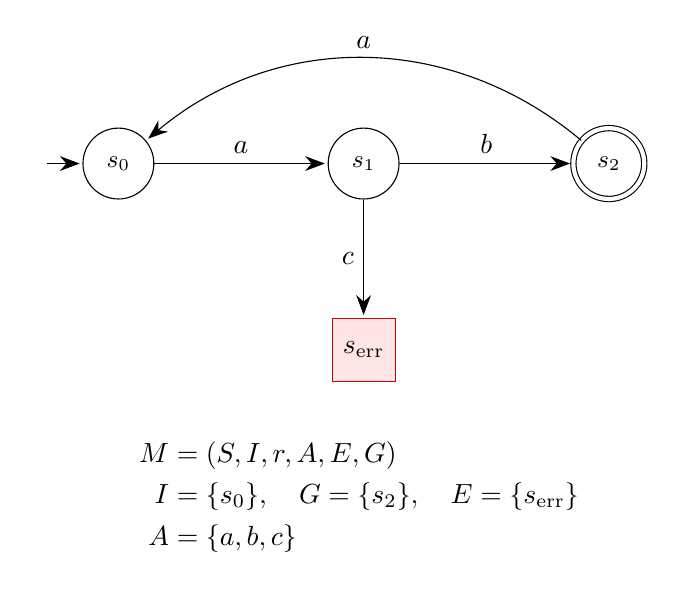
\begin{tikzpicture}[
    shorten >=1pt, node distance=2.2cm, auto,
    >={Stealth[length=2.5mm]},
    state/.style={circle, draw, minimum size=9mm, font=\small},
    initial/.style={initial by arrow, initial text=},
    accepting/.style={double, double distance=1.5pt},
    error/.style={rectangle, draw=red!80!black, fill=red!10, minimum size=8mm}
]

  % States
  \node[state, initial]          (s0) {$s_0$};
  \node[state]                  (s1) [right=of s0] {$s_1$};
  \node[state, accepting]        (s2) [right=of s1] {$s_2$};
  \node[error]                  (se) [below=1.5cm of s1] {$s_{\text{err}}$};

  % Transitions (Relation r)
  \path[->] 
    (s0) edge node {$a$} (s1)
    (s1) edge node {$b$} (s2)
         edge node[left] {$c$} (se)
    (s2) edge[bend right=40] node[above] {$a$} (s0);

  % Annotations / Legend dynamically positioned below error state
  \node[below=0.6cm of se, align=center] (legend) {
    $\begin{aligned}
      M &= (S, I, r, A, E, G) \\
      I &= \{s_0\}, \quad G = \{s_2\}, \quad E = \{s_{\text{err}}\} \\
      A &= \{a, b, c\}
    \end{aligned}$
  };

\end{tikzpicture}
\caption{Transition System $M$ as a State Transition Graph}
\end{figure}

\begin{tcolorbox}[
    enhanced,
    frame hidden,
    borderline west={2pt}{0pt}{black},
    boxsep=5pt,
    left=8pt
]
\textbf{Definition.} A Trace (Trajectory) of the System \textit{M = (S, I, r, A)} is a finite or infinite sequence $s_o, a_0, s_1, a_1, s_2, ...$ starting from $s_o \in I$ with steps given by \textit{r}:

\[
\begin{array}{c@{\quad\quad}l}
  \boxed{s_0} & s_0 \in I \\[0.3em]
  \Big\downarrow a_0 & a_0 \in A \\[0.5em]
  \boxed{s_1} & (s_0, a_0, s_1) \in r \\[0.3em]
  \Big\downarrow a_1 & a_1 \in A \\[0.5em]
  \boxed{s_2} & (s_1, a_1, s_2) \in r \\[0.5em]
  \dots & 
\end{array}
\]

In general, we require $(s_i, a_i, s_{i+1}) \in r$ for all \textit{i} in the length of the sequence. If the trace is finite, we assume it ends with a state $s_n$ and call \textit{n} its length. \\

\textit{Traces(M)} is the set of all traces of \textit{M}. 
\end{tcolorbox}


\section*{Reach}

\begin{tcolorbox}[
    enhanced,
    frame hidden,
    borderline west={2pt}{0pt}{black},
    boxsep=5pt,
    left=8pt
]
\textbf{Definition.} \textit{Reach(M)}: reachable states $s_n$ for which there exists a trace that ends in $s_n$. 
\[
	\text{Reach(M)} = \{s_n \, | \, \exists \textbf{n}. \exists (s_o, a_o, s_1, a_1, ..., s_n) \in \text{Traces(M)} \} 
.\] 
\end{tcolorbox}

\subsection*{Explicit-State Reachability Checking}
The goal is to determine whether an \textbf{error state} \textit{E} is reachable from any initial state \textit{I} in a finite-state transition system \textit{M = (S, I, r, A)}.

\begin{itemize}
	\item Input: \textit{M = (S, I, r, A)}, where \textit{S} is \textbf{finite}, $E \subseteq S$ (error states)
	\item Output: either a $(s_0, a_0, s_1, a_1, ..., s_n) \in$ \textit{Traces(M)} where $s_n \in E$, or the answer "Safe" if no such trace exists.
	\item Idea: graph reachability from nodes in \textit{I}, following edges in ($s, a, s'$) $\in r$ as long as we have not seen $s'$ before. 
	\item To be able to report the trace, build a directed reachability graph of explored edges (never create cycles or duplicate nodes)
	\item If no edge in \textit{r} leads to a previously unexplored node, we stop (this must eventually happen because \textit{S} is finite). 
	\item \textbf{Graph search implementation}: \underline{graph reachability using a work list}. For efficiency, define three sets of nodes in a graph. Key operation: from frontier node \textit{s}, add all of it's unexplored non-frontier successors to the frontier, move \textit{s} to explored. 
	\begin{itemize}
		\item Set of all nodes
		\item Explored nodes: whose all successors we have explored
		\item Frontier nodes (worklist): we have explore them but not their successors. 
	\end{itemize}
	
\end{itemize}

\newpage
\section*{Exercise 1: Bounded Counter}

Consider a system with $S = \{0, 1, 2, ..., 6\}$ that takes signals $A = \{+, -\}$ with initial state 0 and count up by 2 on + and down by 2 on - but never goes below 0 or above 6 (stays in the state if needed). Write down the transition system definition and prove that the state $E = \{3\}$ is not reachable using explicit-state reachability algorithm. Draw the reachability graph. 

\begin{figure}[H]
\centering
\begin{tikzpicture}[
    shorten >=1pt, node distance=2.2cm, auto,
    >={Stealth[length=2.5mm]},
    state/.style={circle, draw, minimum size=9mm, font=\small},
    initial/.style={initial by arrow, initial text=},
    accepting/.style={double, double distance=1.5pt},
    error/.style={rectangle, draw=red!80!black, fill=red!10, minimum size=8mm}
]

  % States
  \node[state, initial]         (0) {0};
  \node[state]                  (2) [right=of 0] {2};
  \node[state]                  (4) [right=of 2] {4};
  \node[state]                  (6) [right=of 4] {6};
  \node[error]                  (1) [below=1.5cm of 0] {1};
  \node[error]                  (3) [below=1.5cm of 2] {3};
  \node[error]                  (5) [below=1.5cm of 4] {5};

  % Transitions (Relation r)
  \path[->]
    (0) edge[bend left=15] node {+2} (2)
    (2) edge[bend left=15] node {-2} (0)
    (2) edge[bend left=15] node {+2} (4)
    (4) edge[bend left=15] node {-2} (2)
    (4) edge[bend left=15] node {+2} (6)
    (6) edge[bend left=15] node {-2} (4)
    (1) edge[bend left=15] node {+2} (3)
    (3) edge[bend left=15] node {-2} (1)
    (3) edge[bend left=15] node {+2} (5)
    (5) edge[bend left=15] node {-2} (3);

  % Annotations / Legend dynamically positioned below error state
  \node[below=0.8cm of 5, align=center] (legend) {
    $\begin{aligned}
      M &= (S, I, r, A, E) \\
      r &= $\{(0, +, 2), (2, +, 4), (4, +, 6), \\
	& (2, -, 0), \, (4, -, 2), \, (6, -, 4), \\ 
	& (1, +, 3), \, (3, +, 5), \, (3, -, 1), \, (5, -, 3) \}$ 

    \end{aligned}$
  };

\end{tikzpicture}
\caption{$Reach(M) = \{0, 2, 4, 6\} \, and \, E = \{1, 3, 5\} \Rightarrow Reach(M) \cap E = \emptyset$}
\end{figure}

\section*{Simplified Transition Relation and Reachable States}

\textbf{Idea:} ignore the environment signals defined by $a$. Hence, we consider all possible transitions from $s$ to $s'$, keeping only the connection between states: 

\begin{tcolorbox}[
    enhanced,
    frame hidden,
    borderline west={2pt}{0pt}{black},
    boxsep=5pt,
    left=8pt
]
Let $M = (S, I, r, A)$ be a transition system. \\
\textbf{Definition.} $\bar{r} = \{(s, s') \, | \, \exists a \in A. (s, a, s') \in r\}$ \\

Note: even if \textit{r} is deterministic, $\bar{r}$ can become non-deterministic. \textit{\underline{Reminder}}: a relation is non-deterministic when a state has multiple possible next states. Removing action labels can combine transitions that were distinguished by their actions. \\ 

\textbf{Counter ex.: } $\bar{r} = \{ (0, 2), (2, 4), (2, 0), (4, 6), (4, 2), (6, 4)\}$

\end{tcolorbox}

\begin{tcolorbox}[
  colback=green!15,     % background color
  colframe=black!50,    % border color
  boxrule=1pt,       % border thickness
  arc=3mm,             % rounded corners
  left=4mm, right=4mm, top=2mm, bottom=2mm % padding
]
Composition of relations: $r_1 \circ r_2 = \{ (x, z) \, | \, \exists y.(x, y) \in r_1 \land (y, z) \in r_2\}$ \\
Iteration (paths of length \textit{n}): $r_1^{0} = \Delta = \{(x,x) \, | \, x \in A\}, \quad r_1^{n+1} = r_1 \circ r_1^{n}$ 
\begin{itemize}
	\item $r^{0} = \Delta$: paths of length zero. Every state reaches itself without taking a step. 
	\item $r^{1} = r$ paths of one step. 
	\item $r^{n}$: paths of exactly n steps.
	\item $r^{*}$: paths of any finite length, including zero. 
\end{itemize}

Transitive closure of $r_1$: 
\[
	r_1^{*} = \bigcup_{n \geq 0} r_1^{n} \quad \text{relates endpoints of all finite paths in graph given by} \, r_1
.\] 

Image of a set under relation: $r_1[X] = \{y \, | \, \exists x \in X.(x,y) \in r_1\}$. This simply means: \textbf{find every state that can be reached in one step from a state in \textit{X}}. \textit{Counter ex.:} $\bar{r}[X] = \{0, 2, 4\}$ since from 0 we can reach 2, from 2 we can reach 0 and 4. 
\end{tcolorbox}

\textcolor{blue}{Theorem}

\textit{Reach(M)} = $(\bar{r}) * [I]$ (\textit{end points of all finite paths starting in I)}. Intuitively, this means that \textit{Reach(M)} are the states collected by all arbitrary long paths where pairs are precisely the image of the set \textit{I} under the transitive closure. 

We can also define \textit{post(X)} = $\bar{r}[X]$ if $X \subseteq S$ under the system $M = (S, I, r, A)$. It means \textbf{all immediate successors of the states in \textit{X}}.

$\Rightarrow$ $\text{post}^{0}(X) = X, \, \text{post}^{n+1}(X) = \text{post}(\text{post}^{n}(X))$

\textbf{Counter ex.:} starting from $I = \{0\}$: 
\begin{itemize}
	\item $\text{post}^{0}(I) \Rightarrow \{0\}$ \textit{Initial states}
	\item $\text{post}^{1}(I) \Rightarrow \{2\}$ \textit{Reachable in one step}
	\item $\text{post}^{2}(I) \Rightarrow \{0, 4\}$ \textit{Reachable in two steps}
	\item $\text{post}^{3}(I) \Rightarrow \{2,6\}$ \textit{Reachable in three steps}
\end{itemize}


\textcolor{blue}{Theorem}

\[
	\bigcup_{n \geq 0} \text{post}^{n}(I) = \text{Reach(M)}
.\] 

\section*{Invariant}

\begin{tcolorbox}[
    enhanced,
    frame hidden,
    borderline west={2pt}{0pt}{black},
    boxsep=5pt,
    left=8pt
]
\textbf{Def.} \textbf{Invariant} \textit{P} of the system \textit{M} is any superset of reachable states: $Reach(M) \subseteq P$. 
\begin{itemize}
	\item \textit{P} is a property satisfied by all reachable states (though not all states in \textit{P} need to be reachable). 
	\item In every trace, by definition $s_i \in \text{Reach(M)} \subseteq P$. So the property $s_i \in P$ remains in-variant (does not change) as the system makes a step from \textit{i} to \textit{i + 1}. 
\end{itemize}
\end{tcolorbox}

\textbf{Example: the counter is always even}. Consider $P = \{ s \in S \, | \, \text{s is even} \}$. We found that \textit{Reach(M) = \{0, 2, 4, 6\}} and we have that \textit{P = \{0, 2, 4, 6\}}. Since every reachable state is in \textit{P}, this is an invariant. Note that \textit{P = \{0, 1, 2, 3, 4, 5, 6\} = S} is also an invariant because all reachable states are in \textit{S}.  

\section*{Inductive invariant}

\textcolor{blue}{This is one of the most important concepts in formal verification because it lets us prove properties without enumerating every reachable state}. 

\begin{tcolorbox}[
    enhanced,
    frame hidden,
    borderline west={2pt}{0pt}{black},
    boxsep=5pt,
    left=8pt
]
\textbf{Def.} \textbf{Inductive invariant} \textit{Ind} is a set of states $\text{Ind} \subseteq S$ that satisfies the following:
\begin{itemize}
	\item $I \subseteq \text{Ind}$ (holds initially)
	\item if $s \in \text{Ind}$ and $(s, a, s') \in r$, then $s' \in \text{Ind}$. \\
\end{itemize}

In simple terms: start inside the set and never leave the set. If both conditions hold, every reachable state must belong to \textit{Ind}.
\end{tcolorbox}

\textbf{Example: proving the counter is always even}. Choose \textit{Ind = \{0, 2, 4, 6\}}. Let's verify both conditions:
\begin{itemize}
	\item \textbf{Condition 1 - Initial states}
		\begin{itemize}
			\item The initial state is $0$, and $0 \in \text{Ind}$. Therefore, $I \subseteq \text{Ind}$ holds.
		\end{itemize}
	\item \textbf{Condition 2 - Transitions}. \\
		Check every transition from a state in \textit{Ind}:
		\begin{itemize}
			\item $0 \rightarrow 2$: remains in \textit{Ind}
			\item $2 \rightarrow 0$ and $2 \rightarrow 4$: remain in \textit{Ind}
			\item $4 \rightarrow 2$ and $4 \rightarrow 6$: remain in \textit{Ind}
			\item $6 \rightarrow 4$: remains in \textit{Ind}.
\end{itemize}
	Therefore, no transition leaves \textit{Ind}.
\end{itemize}

We proved the result by checking the initial state and the transitions, rather than exploring every possible trace. 
\end{document}
